\chapter{Infraestrutura}
%Foi possível demonstrar uma aplicação que escala sob demanda
%Foi apresentada uma arquitetura que é possível de ser aplicada em produção

\section{Uso da infraestrutura}

A escolha da infraestrutura para a solução final foi o uso da
computação em nuvem (\autoref{infraestrutura-em-nuvem}), visto que, proporciona
escalabilidade que o problema exige - uma das principais vantagens da computação em nuvem.
Além é claro, do baixo custo inicial que a aplicação terá antes de começar a gerar qualquer
tipo de lucro.

Conforme discutido a respeito das topologias das plataformas em
nuvem (\autoref{tipologia-das-plataformas-em-nuvem}), para a solução final foi escolhido o
modelo IaaS (\autoref{iaas}) que fornece a opção de rodar programas como Docker e
Kubernetes, tornando a escolha do serviço de plataforma em nuvem independente da forma
com que o software roda. Ou seja, há um desacoplamento da infraestrutura com o software
(\autoref{ferramentas}).

\section{Análise de desempenho}

Foram feitos vários testes em cima do serviço de reserva de ingressos que foi implementado
(\autoref{implementacao-do-servico}) para saber quais eram seus limites.
É importante deixar claro que a análise ocorrera em um notebook pessoal com poder
de processamento limitado. Em um ambiente real (nuvem \autoref{infraestrutura-em-nuvem})
poderão existir diversas máquinas disponíveis para que sejam utilizadas
(escalabilidade horizontal \autoref{escalabilidade})
permitindo que os números exibidos abaixo sejam muito maiores.

\subsection{Gatling: ferramenta para geração da análise de desempenho}

Os testes de perfomance realizados em cima da aplição de reserva de ingressos foram
feitos com a ferramenta Gatling na versão 2.3.
Com a ferramenta é possível testar alta performance de aplicações web
\cite{gatling-docs} que seguem o protocolo HTTP.

\subsection{@@Gráficos da análises de desempenhos}

O teste de performance de requisições foi feito usando a
estratégia do método heavisideUsers \cite{gatling-simulation-setup}
que o Gatling possui, simulando assim a utilização simultânea do sistema por
grande quantidade de usuários.
Todas as requisições da análise foram configuradas para serem executadas no período
de 10 segundos.
Os testes foram feitos para medir a degradação do sistema em relação ao aumento do
número de requisições simulando um ambiente onde haveriam muitas requisições para
reserva de ingressos.
Com a degração do sistema as respostas começam a demorar mais, ou seja,
o teste demora mais para ser finalizado conforme o aumento do número de requisições.
Com isso, o único parâmetro que muda de um teste para o outro
é o número de requisições realizadas.
Todos os resultados com todos os testes realizados pode ser consultados de maneira
iterativa através do link \url{https://andreformento.github.io/term-paper/index.html}.

Na \autoref{03000-requests-config-10s-duration-10} são feitas 3000 requisições apenas.
O sistema responde todas elas com sucesso e um desvio padrão de 241 milisegundos
para o tempo de respostas das requisições.
97\% das requisições respondem em menos de 800 milisegundos e apenas 3\% das requisições
respondem em até 1200 milisegundos.

\begin{figure}[h]
  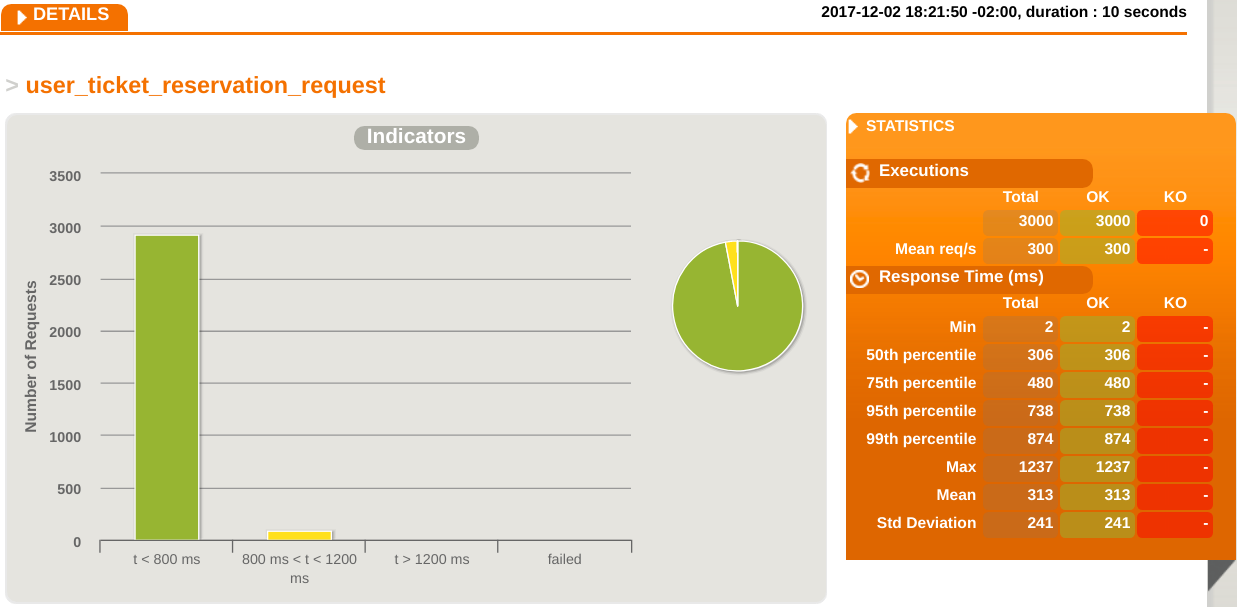
\includegraphics[width=\textwidth]{03000-requests-config-10s-duration-10}
  \caption{Dados do Gatling com 3000 requisições executados em 10 segundos}
  \label{03000-requests-config-10s-duration-10}
\end{figure}


\section{@Trabalhos futuros}\label{trabalhos-futuros}

@@ Implementação de outros serviços; Implementação do frontend
